\section{Problems}

\subsection{title}

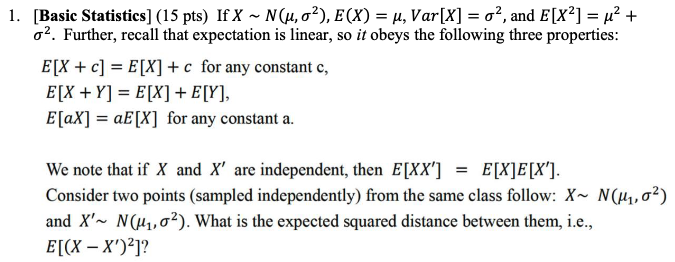
\includegraphics[width=1\textwidth]{media/hw2_q1.png}

\subsection{[Basic Linear Algebra] (15 pts) We are given a vector $x = [0, 0.2, 1.0, 2.2]$. Which of the following vector is closest to $x$ and what is the distance from the closest point to $x$ under each of the following vector norms?}

$$x_1 = [0.7, 0.2, 0.5, 2.0]$$
$$x_2 = [0, 1.0, 1.5, 2.2]$$
$$x_3 = [0.8, 0.1, 1.2, 2.0]$$

a) 0-norm =
b) 1-norm =
c) 2-norm =
d) $\infty$-norm =

\subsection{title}

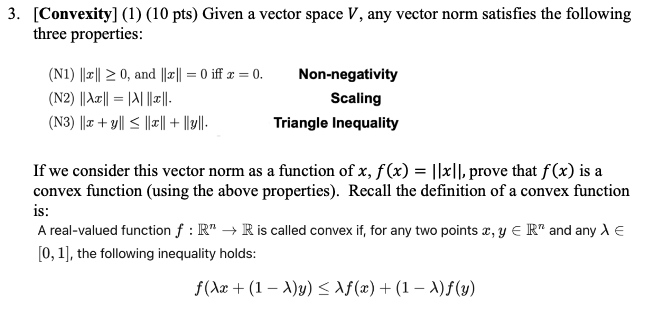
\includegraphics[width=1\textwidth]{media/hw2_q3.png}

\subsection{(2) (10 pts). Prove that the convexity is preserved under a linear transformation. Supposed $f(w)$ is convex in terms of $w$. Prove that $g(w)=f(X w + b)$ is also convex in terms of $w$ where $X$ is a fixed matrix of appropriate size, and $b$ is a fixed vector of appropriate size. (So $X$ and $b$ are not variables in $g$). (Hint: you can simply use the definition of convex function)}

\subsection{(3) (10 pts). From (1) and (2), prove the “loss” function $||y-Xw||_2$ is convex in terms of $w$ where $X_{n \times d}$ is a data matrix containing $n$ examples and each example has $d$ features, and $y$ is a column vector of length $d$. This dataset has been observed and thus
fixed, and $w$ is the only variable in the norm.}